\documentclass{article}
\usepackage[fleqn]{amsmath}
\usepackage{amssymb,graphicx,color,graphicx,slashed, microtype, parskip, enumitem, extarrows, needspace}
%\usepackage[utf8x]{inputenc}
\usepackage[top=1.5cm, bottom=1.5cm, right=6cm, left=1.5cm, heightrounded, marginparwidth=5cm, marginparsep=0.5cm]{geometry}

\hbadness = 10000
\hfuzz=100pt 
    
\usepackage{marginnote}
\renewcommand*{\marginfont}{\footnotesize}

\usepackage{hyperref}
\hypersetup{colorlinks=true, urlcolor=NavyBlue, bookmarksdepth=3}

\makeatletter\newcommand{\@minipagerestore}{\setlength{\parskip}{\medskipamount}}\makeatother

% =============== Index ===========================

\usepackage[nonewpage]{imakeidx}
\makeindex

% =============== Color Definitions ===============
    
\usepackage[svgnames]{xcolor}
\colorlet{ColorTitle}{Black}
\colorlet{ColorSectionName}{Black}
\colorlet{ColorBoxFG}{Gray}
\colorlet{ColorBoxText}{Black}
\colorlet{ColorBoxBG}{White}


% =============== Title Style ===============
    
\usepackage{titling} % Allows custom title configuration
    
\newcommand{\HorRule}{\color{ColorTitle}\rule{\linewidth}{1pt}} % Defines the gold horizontal rule around the title
    
\pretitle{
    \vspace{-50pt} % Move the entire title section up
    \HorRule\vspace{9pt} % Horizontal rule before the title
    \fontsize{27}{36}\usefont{OT1}{phv}{b}{n}\selectfont
    \color{ColorTitle} % Text colour for the title and author(s)
}
    
\posttitle{\par\vskip 15pt} % Whitespace under the title
    
\preauthor{\fontsize{17}{0}\usefont{OT1}{phv}{m}{n}\selectfont\color{ColorTitle}} % Anything that will appear before \author is printed
    
\postauthor{\par\HorRule}

\newcommand{\COURSENAME}{\href{http://phyw.people.ust.hk/teaching/PHYS2022-2015/}{\textcolor{black}{PHYS 2022}}}
\newcommand{\YW}{\href{http://phyw.people.ust.hk/}{\textcolor{black}{Yi Wang}}}
\newcommand{\PHYS}{\href{http://physics.ust.hk}{\textcolor{black}{Department of Physics}}}
\newcommand{\HKUST}{\href{http://www.ust.hk/}{\textcolor{black}{HKUST}}}
\author{\COURSENAME, \YW, \PHYS, \HKUST}

\date{}

% =============== Section Name Style ===============
    
\usepackage{titlesec}
    
\titleformat{\section}
    {\fontsize{15}{20}\usefont{OT1}{phv}{b}{n}\color{ColorSectionName}}
    {\thesection}{1em}{}
    %[{\vspace{0.2cm}\titlerule[0.8pt]}]
    
\titleformat{\subsection}
    {\fontsize{14}{20}\usefont{OT1}{phv}{m}{n}\color{ColorSectionName}}
    {\thesubsection}{1em}{}
    
\titleformat{\subsubsection}
    {\fontsize{12}{20}\usefont{OT1}{phv}{m}{n}\color{ColorSectionName}}
    {}{0em}{}
      
\setcounter{secnumdepth}{4}
        
% =============== Box Style ===============
    
\usepackage[most]{tcolorbox}
    
\newtcolorbox{tbox}[1]{
    colback=ColorBoxBG, colframe=ColorBoxFG, coltext=ColorBoxText,
    sharp corners, enhanced, breakable, parbox=false,
    before skip=1em, after skip=1em,
    title={#1}, fonttitle=\usefont{OT1}{phv}{b}{n}, 
    attach boxed title to top left={yshift=-0.1mm}, boxed title style={sharp corners, colback=ColorBoxFG, left=0.405cm},
    rightrule=-1pt,toprule=-1pt, bottomrule=-1pt
}

\newtcolorbox{mtbox}[1]{
    colback=ColorBoxBG, colframe=ColorBoxFG, coltext=ColorBoxText,
    sharp corners, enhanced, breakable, parbox=false,
    before skip=1em, after skip=1em,
    title={#1}, fonttitle=\usefont{OT1}{phv}{b}{n},
    attach boxed title to top left={yshift=-0.1mm}, boxed title style={sharp corners, colback=ColorBoxFG, left=0.15cm},
    rightrule=-1pt,toprule=-1pt, bottomrule=-1pt, 
    left=0.5em
}

% =============== tikz has to be loaded after xcolor
\usepackage{tikz}

\newcommand*\enumlabel[1]{\tikz[baseline=(char.base)]{
			\node[shape=rectangle,inner sep=2pt,fill=ColorBoxFG] (char) 
			{\fontsize{7}{20}\usefont{OT1}{phv}{b}{n}{\textcolor{ColorBoxBG}{#1}}};}}

% =============== Useful shortcuts ===============

\newcommand\wref[1]{{\hypersetup{linkcolor=white}\ref{#1}}}  

\newcommand{\textbox}[2]{
    \begin{tbox}{#1}
        #2
    \end{tbox}
}

\newcommand{\mtextbox}[2]{\marginnote{
    \begin{mtbox}{#1}
        #2
    \end{mtbox}}
}

\newcommand{\mnewline}{\vspace{0.5em}\newline}

\newcommand{\titem}[1]{
    \begin{itemize}[label=\color{ColorBoxFG}$\blacktriangleright$, leftmargin=0mm, labelsep=0.27cm, topsep=0.5em
        %, itemsep=1ex
        ]
        #1
    \end{itemize}
}

\newcommand{\mtitem}[1]{
    \begin{itemize}[label={\color{ColorBoxFG}$\blacktriangleright$}, leftmargin=0mm, labelsep=1mm, topsep=0.5em
        %, itemsep=1ex
        ]
        #1
    \end{itemize}
}

\newcommand{\itembox}[3]{
    \begin{tbox}{#1}
        #2
        \titem{#3}
    \end{tbox}
}

\newcommand{\mitembox}[3]{
    \marginnote{
    \begin{mtbox}{#1}
        #2
        \mtitem{#3}
	\end{mtbox}
    }
}

\newcommand{\tenum}[1]{
    \begin{enumerate}[label=\protect\enumlabel{\arabic*}, leftmargin=0mm, labelsep=0.265cm, topsep=0.5em
        %, itemsep=1ex
        ]
        #1
    \end{enumerate}
}

\newcommand{\enumbox}[3]{
    \begin{tbox}{#1}
        #2
        \tenum{#3}
    \end{tbox}
}

\newcommand{\twocol}[5]{
    \begin{minipage}[t][][b]
        {#1\textwidth}
        #4        
    \end{minipage}
    \hspace{#2\textwidth}
    \begin{minipage}[t][][b]
        {#3\textwidth}
        #5
    \end{minipage}
}

\newcommand{\cg}[2]{
    \begin{center}
        \includegraphics[width=#1\textwidth]{#2}
    \end{center}
}

\newcommand{\tbar}{
    ~\newline
    {\color{ColorBoxFG}
    \hbox to 0.15\textwidth{\leaders\hbox to 5pt{\hss  \hss}\hfil} 
    \hbox to 0.7\textwidth{\leaders\hbox to 5pt{\hss . \hss}\hfil}}
    \mnewline
}

% =============== Filter unwanted warnings
\usepackage{silence}
\WarningsOff[tcolorbox]
\hbadness=1000000


\graphicspath{{3_fig/}}
\title{Part 3. Cosmology}

\begin{document}

\maketitle

\textbox{The comprehensible universe}{
    The universe is the most complicated object in our universe, since it contains all complexities of all objects in our universe. However, amazingly, Einstein says: 

    ``The most incomprehensible thing about the world is that it is comprehensible.''

    Here let us try to understand the following questions:

    \tenum{
        \item Before understanding everything in the universe, how can we understand anything about the universe, since it is the most complicated?
        \item Why 
        \mtextbox{Other ways to Olbers paradox}{
            The Olbers paradox can also be understood in other equivalent ways, less obvious but may be more insightful:
            \mtitem{
                \item Within an infinitesimal solid angle cone along your line of sight, a star is as bright as the sun. The sun is overall brighter because it spans more solid angle. If the universe is infinite, sooner or later the cone along your line of sight will reach a surface of a star. Thus you will see the sky everywhere as bright as the sun. 
                \item If the universe is static and has infinite duration, we will reach equilibrium with the stars thus the earth is as hot as the star surface. 
            }
        }
        is the night sky dark? 
        
        This question looks stupid, as we are not under sunshine at night. However, what about stars? Why doesn't the night sky appear as bright as daytime under the shining of the stars? 

        You may answer: they are far away. Thus their apparent luminosity decays as $1/r^2$. So they are not as bright as the sun.

        Correct. However, how many stars are there at distance $r$? If our universe is homogeneous and infinite in space and time, statistically, the number of stars at distance $r$ should scale as $r^2$. So why doesn't their light sum up and being as bright as the sun?

        This question is known as the Olbers' paradox (Digges 1576, Olbers 1823).
    }
}

\section{The dynamics of the universe} \label{sec:dynamics-universe}

\textbox{The cosmological principle}{
    To make the universe simpler, let's assume:

    Our universe is approximately homogeneous and isotropic on large scales. 

    This is known as the cosmological principle. 
}

The cosmological principle had already appeared in Newton's \textit{Principia} (1687). However, the study of cosmology in Newtonian mechanics is full of paradoxes. The framework of modern cosmology is setup based on Einstein's general relativity.

In this section, we will still use Newtonian mechanics to set up the theory of our universe with special care. The subtleties in the discussion can be checked in general relativity.

\textbox{Distant galaxies are leaving us}{
    In the 1920s, Hubble (see also Lemaitre and other astronomers' contribution) measured the spectrum of light from other galaxies. As we know the spectrum at emission (recall the characteristic spectrum by atoms), by measuring the observed spectrum, one can find out the velocity of these galaxies along the line of sight direction via Doppler-like effects.

    The result shows that the distant galaxies are leaving us. 
}

\mtextbox{Faster than light?}{
    Is the expansion of the universe faster than light? To be more precise, for distant enough object can they leave us at a rate faster than light?
    \tcblower
    Yes or no. That depends on how to define speed in general relativity. 
    \mnewline
    If you define speed as $dR(t)/dt$, then for distant enough objects, they are indeed leaving us at a speed faster than light. This is not due to the objects themselves moving fast, but instead the emerging space between objectss. This is not contradictory with special relativity, since the speed between two near-by objects (where special relativity applies) cannot be faster than light. 
    \mnewline
    If you define speed as the speed of the moving object (pecular velocity), excluding the expansion of space, then the speed of distant objects are still bounded by the speed of light.
}
\textbox{From the Copernicus principle to the expanding universe}{
    Since Copernicus, human start to realize that the universe does not have a center. However, if all the distant galaxies are moving away from us, does that mean we are at the center of the universe? 

    Not necessarily. Imagine an expanding membrane, or balloon. Wherever you are on the membrane or balloon, you find your neighbor points leaving you. Thus, we can interpret the observation as that the universe is expanding.

    Now that the universe is expanding, how is the expansion rate determined?
    \tcblower
    Let's imagine a universe filled with pressureless dust.    
    The dust particles expand together with the universe expansion, without additional motion by themselves (i.e. comoving, i.e. without peculiar motion).

    \cg{0.35}{cosmo_sphere}

    To quantify the expansion rate of the universe in the framework of Newtonian mechanics, define two set of distances: comoving distance and physical distance.    
    \titem{
        \item The physical distance $R(t)$ is the real distance between two objects, corresponding to actual physical measurements.
        \item The comoving distance $r$ is measured by an expanding coordinate system, such that the comoving dust particles have fixed (i.e. time-independent) coordinate value in the comoving coordinates.
    }
    The comoving coordinate is related to the physical coordinate by
    $
        R(t) = a(t) r,
    $
    where $a(t)$ is known as the \emph{scale factor}, quantifying the time dependence of the universe. The expansion rate of the universe is quantified by the Hubble parameter:
    \begin{align}
        H(t) \equiv \frac{\dot a}{a} ~.
    \end{align}
}

\needspace{0.2\textheight}
\mtextbox{Dust and radiation}{
    As examples, we note that 
    \mtitem{
        \item Pressureless dust: $p=0$. Solving \eqref{eq:continuous}, we get $\rho \propto a^{-3}$. The particle density is diluted as $a^{-3}$, and the energy per particle is a constant.
        \item Radiation: The photon density $\propto a^{-3}$. However, the wavelength of each photon is stretched as $\lambda \propto a$. Thus the energy per photon is proportional to $1/a$ (quantization condition). As a result, $\rho \propto a^{-4}$. This corresponds to $p=\rho/3$. 
    }
    As radiation gets diluted faster than dust, our universe transited from radiation domination to dust domination during its expansion.
}
\textbox{The universe tells matter how to get diluted}{
    Consider a component in the universe (for example, radiation or dust particles) with energy density $\rho$ and pressure $p$. How does $\rho$ evolve with time?
    
    The first law of thermodynamics is $dE = TdS - pdV$. The expansion of the universe is adiabatic since heat will not be conducted in a homogeneous universe. Thus $dS=0$. We have, during the expansion of the universe, $dE/dt = p dV/dt$. Here $V$ is a physical volume $V\propto a^3$. Thus,
    \begin{align}\label{eq:continuous}
        \frac{d(a^3\rho)}{dt}  = p \frac{da^3}{dt}
        \qquad\Rightarrow\qquad
        \dot \rho + 3H (\rho +p) = 0~.
    \end{align}
    This is known as the continuity equation in cosmology, telling that how matter gets diluted during the cosmic expansion.
}

\textbox{What's the matter in the universe?}{
    We know only 5\% of our universe (weighted by their energy composition). Below is a figure indicating what we know and what we don't know.
    \cg{0.8}{components}
    \mtextbox{Einstein's ``biggest mistake''}{
        When Einstein first used general relativity to study our universe, he found that the universe will either expand or contract. He did not like the situation. To keep the universe static as he likes, he added a cosmological constant to his equations (1917). After Hubble discovered the expansion of the universe in the 1920s, Einstein regreted that he had missed the chance to predict an expanding universe, and considered the introduction of the cosmological constant the biggest mistake in his life (1931). However, in 1998, dark energy is discovered, and by far the simplest candidate is the cosmological constant (with a different value, which does not make the universe static but make it expanding with positive acceleration).
    }                     
    \titem{
        \item The matter that we know: Matter made by nucleus and electrons (either in the phase of atoms or plasmas) takes 5\% of the energy burget of our universe. Most of these atoms and plasmas are in the form of free Hydrogen and free Helium. A small part forms stars. Among the matter that we know, the weight of light also takes a tinny part (0.005\%).
        \item The matter that we don't know: observations indicate that there are dark matter (takes about 25\%) and dark energy (takes about 70\%) in the universe. We don't know what are they. But from observations, we know approximately their nature: the dominate part of dark matter is almost pressureless with $p\sim 0$, similar to that of atomic matter now, and contribute attractive gravitational force. However, dark energy has negative pressure $p\sim -\rho$, which effectively provide repulsive gravitational force and is driving an accelerated expansion phase of our universe.
    }
}

\textbox{Matter tells the universe how to expand}{
    To determine the dynamics of $a(t)$, we consider a dust particle with mass $m$, located at comoving distance $r$ (and thus physical distance $R(t)=a(t)r$). The energy conservation equation for this particle is
    \begin{align}\label{eq:pre-friedmann-1}
        \frac{m}{2} \left ( \frac{dR}{dt}  \right)^2 - \frac{GMm}{R} = E = \mathrm{constant}~.
    \end{align}
    The constant $E$ is determined by the initial condition of the universe. Observations tell that $E\simeq 0$ thus we will ignore it (but do not ignore the question why $E\simeq 0$).

    Here $M$ is the mass
    \mtextbox{What about the mass outside?}{
        One can argue that the mass outside the sphere has no force on our particle $m$, since the force cancel for each spherical cell. In fact, the statement depends on the boundary condition of the universe. This is the limitation of the Newtonian cosmology. One needs general relativity to remove this boundary condition dependence.
        }
    inside the sphere:
    \begin{align}\label{eq:pre-friedmann-2}
        Mc^2 = \frac{4\pi R^3}{3} \rho~.
    \end{align}
    Inserting \eqref{eq:pre-friedmann-2} into \eqref{eq:pre-friedmann-1}, we get the Friedmann equation telling the universe how to expand:
    \begin{align}\label{eq:friedmann}
        H^2 = \frac{8\pi G \rho}{3c^2}~.  
    \end{align}
    In Newtonian cosmology, we cannot deal with $p\neq 0$. This is because Newtonian gravity does not define how pressure contribute to gravity. Thus in the above derivation, we used a dust-filled universe. In general relativity, one can verify that \eqref{eq:friedmann} actually also holds for $p\neq 0$, for example a radiation filled universe.
    
    As solutions of \eqref{eq:friedmann}, for a dust-dominated universe, $a(t)\propto t^{2/3}$ and for a radiation-dominated universe, $a(t)\propto t^{1/2}$. We will leave the details to an exercise.
}

\textbox{The age of the universe}{
    We observe that for dust and radiation dominated universes, at $t\rightarrow 0$, the scale factor approaches zero and thus the energy density diverges. 
    \marginnote{For recent estimates of the universe, in 2012 the WMAP experiment estimated that the universe is 13.77 billion years old; and in 2018, the Planck experiment estimated that the universe is 13.8 billion years old. }
    We thus consider $t=0$ as the start of the universe. More detailed study of the very early universe changes this starting point a bit but not very much.

    For a matter dominated universe, from the definition of the Hubble parameter, we have $t=2/(3H)$. To include the observed dark energy (a component with $p=-\rho$), the age of the universe is corrected to approximately $t\simeq 1/H$. Thus, the age of the universe is closely related to the Hubble parameter -- the expansion rate of the universe.
}

\section{The early universe}

When
you are looking deep into the night sky, you are looking through the history, since the star lights may take years, or tens of thousands of years. Modern telescopes can extend this record greatly, to billions of years. What does the early universe look like?

\mtextbox{Is energy conserved in cosmology?}{
    This is a very tricky question. We can answer it in a few aspects:
    \mtitem{
        \item In cosmology, there is no time translation symmetry, since $a(t)$ depends on time. Thus energy will not arise as a conserved quantity following the Noether theorem.
        \item We still have approximate local energy conservation if restricted to very small space volume and time duration: $\sum_\mu\nabla_\mu T^{\mu\nu}=0$.
        \item The matter energy drops since matter has positive pressure and does work when the universe is expanding.
        \item If the gravitational potential energy is considered together, the answer becomes indefinite since there are multiple ways to define gravitational energy in general relativity. 
        }
    }
\textbox{Thermal history: the earlier, the hotter}{
    The earlier universe is hotter than our current universe. That's because the expansion of the universe stretches the energy per photon. Or you can understand it as that during the expansion the gas does work and thus lose energy.

    The events in the early universe is related to the temperature scales of the universe. Thus, the history of the universe is known as the thermal history.

    It is believed that the very early universe was in a state with a higher temperature than all man-made experiments now and in the forseeable future.

    \tcblower

    Below is a figure about the thermal history of the universe. 

    \begin{center}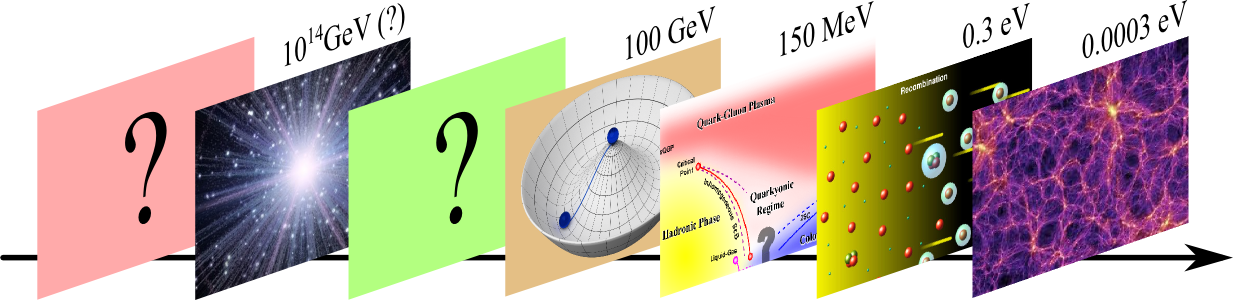
\includegraphics[width=0.8\textwidth]{history}\end{center}

    \titem{
        \item When the universe was 20 picoseconds old (with temperature 100 GeV), a spontaneous symmetry breaking generated mass for known massive fundamental particles.
        \item When the universe was 20 microseconds old (with temperature 150 MeV), free quarks are binded into protons and neutrons. Their binding enery is the main source of mass of atomic matter.
        \item When the universe was 3 minutes old (with temperature 0.1 MeV), light elements, especially helium, are created from protons and neutrons. 
        \item When the universe was 50,000 years old (with temperature 1eV), 
        the universe becomes dominated by non-relativistic matter instead of relativistic radiation.
        \item When the universe was 400,000 years old (with temperature 0.3 eV), the universe become transparent and light for the first time can travel in the universe freely.
        \item In the following billions of years, structures grow in the universe.
        \item Now our universe is about 14 billion years old.
        The universe starts to be dominated by dark energy with $p=-\rho$. We yet need to theoretically and observationally understand the nature of dark energy. 
    }
}

\section{Epilogue: Summary and What's Next}

\textbox{Further reading about the content}{
    \titem{
        \item See Baumann's \href{http://www.damtp.cam.ac.uk/user/db275/Cosmology/Lectures.pdf}{Cosmology} for a detailed introduction of this content.
    }
}

\textbox{What happens next?}{
    Let's first literally discuss what happens next -- what's the future (even fate) of the universe? Now our universe is dominated by dark energy. The energy density of dark energy does not change during the expansion of the universe. As a result, dark energy will become more and more important for the fate of the universe. If the energy density of dark energy is indeed a constant, most galaxies in our present universe will leave our horizon, leaving only $\mathcal{O}(100)$ galaxies around us observable (known as the local group). But we need to further understand dark energy both theoretically and observationally to be more confident about this fate.

    You will find more details about our universe in a course of cosmology. Also, in general relativity there is usually an introduction to cosmology as an application. In-depth study of cosmology usually have close relations to astronomy and high energy physics. 
}

\section{Exercises}

\textbox{E\wref{sec:dynamics-universe}-1 Scale factor as a function of time}{
    For $p=0$ (dust), $p=\rho/3$ (radiation), $p=-\rho$ (dark energy), solve the Friedmann equation to get $a(t)$. Based on your solution, estimate the age of the universe given the value of $H$.
}

\textbox{E\wref{sec:dynamics-universe}-2 The age of our universe}{
    For the energy composition given in the pie diagram of the main text, estimate the age of the universe. You may first have an analytical estimate and then numerically solve the equations to test your estimate.
}

\printindex

\end{document}
